\section{Метрические пространства. Примеры}

\begin{definition}
	$ M $ -- множество, $ \qquad \rho : M \times M \to \R $ \\
	Говорят, что $ (M, \rho) $ -- метрическое пространство, если:
	\begin{enumerate}
		\item $ \rho(x, y) \ge 0, \qquad \rho(x, y) = 0 \iff x = y $
		\item $ \rho(x, y) = \rho(y, x) $
		\item $ \rho(x, y) \le \rho(x, z) + \rho(z, y) $
	\end{enumerate}
	$ \rho $ называется метрикой
\end{definition}

\begin{exmpls}
	\item $ \R, \quad \rho(x, y) = |x - y| $
	\item $ \R^2 $
	\begin{enumerate}
		\item $ \rho_2 \big( (x_1, y_1), (x_2, y_2) \big) = \sqrt{(x_1 - x_2)^2 + (y_1 - y_2)^2} $
		\item $ \rho_1 \big( (x_1, y_1), (x_2, y_2) \big) = |x_1 - x_2| + |y_1 - y_2| $ -- \textbf{манхэттенская} метрика
		\item $ \rho_n \big( (x_1, y_1), (x_2, y_2) \big) = \bigg( |x_1 - x_2|^n + |y_1 - y_2|^n \bigg)^{\frac1n} $ -- является метрикой, если $ p \ge 1 $
		\begin{remark}
			Неравенство треугольника следует из неравенства Минк\'{о}вского:
			$$ \bigg( \sum_i |x_i + y_i|^p \bigg)^{\frac1n} \le \bigg( \sum_i |x_i|^p \bigg)^{\frac1p} + \bigg( \sum_i |y_i|^p \bigg)^{\frac1p} $$
		\end{remark}
		\item $ \rho_\infty \big( (x_1, y_1), (x_2, y_2) \big) = \max\set{|x_1 - x_2|, |y_1 - y_2|} $
	\end{enumerate}
	\item Аналогично для $ \R^n $
	\item $ M $ -- произвольное множество \\
	$ \rho(x, y) =
	\begin{cases}
		1, \quad x \ne y \\
		0, \quad x = y
	\end{cases} $ -- \textbf{дискретная} метрика
	\item $ (M, \rho) $ -- метрическое пространство \\
	$ \rho'(x, y) = \dfrac{\rho(x, y)}{1 + \rho(x, y)} \quad $ или $ \quad \rho'(x, y) = \min\set{\rho(x, y), 1} $ \\
	Теперь $ \rho'(x, y) < 1 $
	\item $ M $ -- множество строчек из 0 и 1 длины $ n $ \\
	$ \rho $ -- количество символов, в которых эти строки различаются
	\item $ M $ -- пространство (хороших) функций на $ [a, b] $
	\begin{enumerate}
		\item $ \rho_1(f, g) = \dint{a}b{|f(x) - g(x)|} $
		\item $ \rho_2(f, g) = \sqrt{\dint{a}b{ \big( f(x) - g(x) \big)^2}} $
		\item $ \rho_p(f, g) = \bigg( \dint{a}b{ \big( f(x) - g(x) \big)^p} \bigg)^{\frac1p} $
		\item $ \rho_\infty = \sup\limits_{x \in [a, b]} |f(x) - g(x)| $
	\end{enumerate}
	\item $ M $ -- множество (хороших) фигур на плоскости
	\begin{enumerate}
		\item $ \rho(F, G) = S_{F \triangle G} $
		\item Метрика \textbf{Хаусдорфа}:
		\begin{multline*}
			\rho(F, G) = \\ = \max\set{\inf\set{\veps | \forall f \in F \quad \exist g \in G : \rho(f, g) \le \veps}, \inf\set{\veps | \forall g \in G \quad \exist f \in F : \rho(f, g) \le \veps}}
		\end{multline*}
	\end{enumerate}
	\item $ \Z $
	\begin{undefthm}{Напоминание}
		$ p \in \Prime, \qquad n = 2^{\alpha_1} \cdot 3^{\alpha_2} \cdot ... \cdot p^{\alpha_k} \qquad v_p(n) \define \alpha_k $
	\end{undefthm}
	Введём норму:
	$$ \norm{n} \define 2^{-v_p(n)} $$
	Теперь можно ввести $ \bm{p} $\textbf{-адическую} метрику:
	$$ \rho_p(a, b) = \norm{a - b} $$
	\begin{remark}
		Это расширяется на $ Q $, если ввести
		$$ v_p(\frac{m}n) \define v_p(m) - v_p(n) $$
	\end{remark}
\end{exmpls}

\section{Внутренние точки в метрическом пространстве. Внутренность}

\begin{definition}
	$ (M, \rho) $ -- метрическое пространство, $ \qquad A \sub M, \qquad x_0 \in M $ \\
	Точка $ x_0 $ называется внутренней для $ A $, если
	$$ \exist \veps > 0 : B(x_0, \veps) \sub A $$
\end{definition}

\begin{definition}
	Множество внутренних точек называется внутренностью
\end{definition}

\begin{notation}
	$ \Int A $
\end{notation}

\begin{definition}
	Множество $ A $ называется открытым, если оно совпадает с $ \Int A $, т. е. не содержит ни одной граничной точки
\end{definition}

\begin{lemma}\label{lm:1}
	Объединение открытых является открытым, т. е.
	$$ \bigcup_{i \in I} U_i \text{ -- откр. } \iff \forall i \quad U_i \text{ -- откр.} $$
\end{lemma}

\begin{proof}
	 $$ x_0 \in \bigcup_{i \in I} U_i \implies \exist i : x_0 \in U_i \underimp{Ui \text{ -- откр.}} \exist \veps : B(x_0, \veps) \sub U_i \implies B(x_0, \veps) \sub \bigcup_{i \in I} U_i $$
\end{proof}

\begin{lemma}\label{lm:2}
	$ B(x_0, \veps) $ открыто
\end{lemma}

\begin{proof}
	Возьмём $ \forall x_1 \in B(x_0, \veps) $ \\
	Положим $ \delta \define \veps - \rho(x_1, x_0) $ \\
	Докажем, что $ B(x_1, \delta) \sub B(x_0, \veps) $:
	$$ \forall x_2 \in B(x_1, \delta) \quad \rho(x_1, x_2) < \delta = \veps - \rho(x_0, x_1) $$
	$$ \rho(x_0, x_2) \trile \rho(x_0, x_1) + \rho(x_1, x_2) < \veps $$
	$$ x_2 \in B(x_0, \veps) $$
\end{proof}

\begin{theorem}\label{th:1}
	Равносильны определения внутренности:
	\begin{enumerate}
		\item \label{en:1} Множество внутренних точек
		\item \label{en:2} $ \bigcup_{
			\begin{subarray}{c}
				U \sub A \\
				U \text{ откр.}
			\end{subarray}} U $
		\item \label{en:3} максимальное открытое подмножество $ A $
	\end{enumerate}
\end{theorem}

\begin{proof}
	\hfill
	\begin{itemize}
		\item \ref{en:2} $ \iff $ \ref{en:3} \\
		Очевидно из леммы \ref{lm:1}
		\item \ref{en:2} $ \implies $ \ref{en:1}
		$$ x_0 \in \bigcup_{
			\begin{subarray}{c}
				U \sub A \\
				U \text{ откр.}
			\end{subarray}} U \sub A \implies \exist \veps > 0 : B(x_0, \veps) \sub \bigcup_{
			\begin{subarray}{c}
				U \sub A \\
				U \text{ откр.}
			\end{subarray}} U \sub A \implies x_0 \text{ -- внутр. т. для } A $$
		\item \ref{en:1} $ \implies $ \ref{en:2}
		$$ x_0 \text{ -- внутр. т. для } A \implies \exist \veps > 0 : \underset{\text{откр.}}{B(x_0, \veps)} \sub A $$
		Применяем лемму \ref{lm:2}
	\end{itemize}
\end{proof}

\section{Граница и замыкание множества в метрическом пространстве}

\begin{definition}
	$ (M, \rho) $ -- метрическое пространство, $ \qquad A \sub M, \qquad x_0 \in M $ \\
	$ x_0 $ называется
	\begin{itemize}
		\item внешней для $ A $, если
		$$ \exist \veps > 0 : B(x_0, \veps) \cap A = \O $$
		\item граничной -- если не внутренняя и не внешняя, т. е. если
		$$ \forall \veps > 0
		\begin{cases}
			B(x_0, \veps) \not\sub A \\
			B(x_0, \veps) \not\sub (M \setminus A)
		\end{cases} $$
	\end{itemize}
\end{definition}

\begin{definition}
	\hfill
	\begin{itemize}
		\item Множество внешних точек называется внешностью
		\begin{notation}
			$ \Ext A $
		\end{notation}
		\item Множество граничных точек называется границей
		\begin{notation}
			$ \Fr A, \quad \delta A $
		\end{notation}
	\end{itemize}
\end{definition}

\begin{definition}
	Объединение внутренности и границы называется замыканием
\end{definition}

\begin{notation}
	$ \Cl A $
\end{notation}

\begin{definition}
	Множество $ A $ называется замкнутым, если оно совпадает с $ \Cl A $, т. е. если $ M \setminus A $ открыто
\end{definition}

\begin{theorem}\label{th:2}
	$ M $ -- метрическое пространство, $ A \sub M $ \\
	Равносильны определения замыкания:
	\begin{enumerate}
		\item\label{en:21} Множество внутренних и граничных точек
		\item\label{en:22} $ M \setminus \Int(M \setminus A) $
		\item\label{en:23} $ \bigcap_{
			\begin{subarray}{c}
				F \supset A \\
				F \text{ -- замкн.}
			\end{subarray}} F $
		\item\label{en:24} Минимальное замкнутое, содержащее $ A $
	\end{enumerate}
\end{theorem}

\begin{proof}
	\hfill
	\begin{itemize}
		\item $ \ref{en:23} \iff \ref{en:24} $ -- очевидно
		\item $ \ref{en:21} \iff \ref{en:22} $
		$$ \Int(M \setminus A) = \Ext A $$
		\item $ \ref{en:22} \iff \ref{en:23} $
		$$ M \setminus \Int(M \setminus A) = M \setminus \bigcup_{
			\begin{subarray}{c}
				U \sub M \setminus A \\
				U \text{ -- откр.}
			\end{subarray}} U \underset{\text{(де Морган)}}= \bigcap_{
			\begin{subarray}{c}
				U \sub M \setminus A \\
				U \text{ -- откр.}
			\end{subarray}} M \setminus U = \bigcap_{
			\begin{subarray}{c}
				F \supset A \\
				F \text{ -- замкн.}
			\end{subarray}} F $$
	\end{itemize}
\end{proof}

\section{Топологические пространства. Задание топологии замкнутыми множествами. Примеры}

\begin{definition}
	$ X $ -- множество, $ \qquad \Omega \sub 2^X $ \\
	$ (X, \Omega) $ называется топологическим пространством, если:
	\begin{enumerate}
		\item $ \forall \set{U_i} \sub \Omega \quad \bigcup U_i \in \Omega $
		\item $ U_1, ..., U_n \in \Omega \implies \bigcap_{i = 1}^n U_i \in \Omega $
		\item $ \O, X \in \Omega $
	\end{enumerate}
	$ \Omega $ называется топологией на $ X $ \\
	$ U \in \Omega $ называется открытым
\end{definition}

\begin{definition}
	$ F $ называется замкнутым, если $ X \setminus F $ -- открыто
\end{definition}

\begin{theorem}
	$ (X, \Omega) $ -- топологическое пространство
	\begin{enumerate}
		\item $ \set{F_i}_{i \in I} $ -- замкн. $ \implies \bigcap_{i \in I} $ замкн.
		\item $ F_1, ..., F_n $ -- замкн. $ \implies \bigcup_{i = 1}^n F_i $ -- замкн.
		\item $ \O, X $ -- замкн.
	\end{enumerate}
\end{theorem}

\begin{proof}
	Уже доказано
\end{proof}

\begin{remark}
	Топологическое пространство можно задавать замкнутыми множествами
\end{remark}

\begin{exmpls}
	\item $ (M, \rho) $ -- метр. $ \implies M $ -- тополог. Открыты те множества, которые были открытыми в $ \rho $
	\item $ X $ -- любое, $ \quad \Omega = \set{\O, X} \quad $ -- \textbf{антидискретная топология}
	\item $ X $ -- любое, $ \quad \Omega = 2^X $ -- \textbf{дискретная топология}
	\item \textbf{``Топология Зарисского'' (топология конечных дополнений)}: \\
	$ X $ -- бесконечно, $ \quad $ замкнутые -- конечные и $ X $
	\item \textbf{Стрелка:} \\
	$ X = \R $ (или $ \R_+ $, или ...) \\
	Открытые -- открытые лучи $ (a, +\infty) $, $ \O $, $ X $
	\begin{note}
		Если открытыми считать замкнутые лучи $ [a, +\infty) $, то это \textbf{не} топология:
		$$ \bigcap_{n \in \N} \bigg[ \frac1n, +\infty \bigg] = (0, +\infty) $$
	\end{note}
	\item \textbf{Топология Зарисского:}
	\begin{enumerate}
		\item $ X = \Co $ \\
		Замкнутым будем называть множество корней некоторого многочлена
	\end{enumerate}
\end{exmpls}

\section{Расположение точки относительно множества в топологическом пространстве}

\begin{definition}
	$ (X, \Omega) $ -- топологическое пространство, $ x_0 \in X $ \\
	Окрестностью $ x_0 $ будем называть любое открытое множество, содержащее $ x_0 $
\end{definition}

\begin{definition}
	$ A \sub X, \qquad x_0 \in X $ \\
	$ x_0 $ называется
	\begin{itemize}
		\item внутренней, если
		$$ \exist \underset{\text{(окр. } x_0)}{U_{x_0}} \sub A $$
		\item внешней, если
		$$ \exist U_{x_0} \cap A = \O $$
		\item граничной, если
		$$ \forall U_{x_0} \quad
		\begin{cases}
			U_{x_0} \not\sub A \\
			U_{x_0} \ne \O
		\end{cases} $$
	\end{itemize}
\end{definition}

\begin{definition}
	\hfill
	\begin{itemize}
		\item $ \Int A $ -- множество внутренних точек
		\item $ \Ext A = \Int(X \setminus A) = $ множество внешних точек
		\item $ \delta A = \Cl A \setminus \Int A $ -- множество граничных точек
	\end{itemize}
\end{definition}

\begin{theorem}
	Равносильны определения внутренности:
	\begin{enumerate}
		\item Множество внутренних точек
		\item $ \bigcup_{U \in \Omega} U $
		\item максимальное открытое подмножество $ A $
	\end{enumerate}
\end{theorem}

\begin{proof}
	Точно так же, как теорема \ref{th:1}
\end{proof}

\begin{theorem}
	Равносильны следующие определения замыкания:
	\begin{enumerate}
		\item $ \Cl A = X \setminus \Ext A $ -- множество внутренних и граничных точек
		\item $ \bigcap_{
			\begin{subarray}{c}
				F \supset A \\
				F \text{ -- замкн.}
			\end{subarray}} F $
		\item минимальное замкнутое, содержащее $ A $
	\end{enumerate}
\end{theorem}

\begin{proof}
	Точно так же, как теорема \ref{th:2}
\end{proof}

\begin{statement}
	$ U $ -- откр., $ \quad F $ -- замкн. \\
	Тогда $ U \setminus F $ -- откр., $ \quad F \setminus U $ -- замкн.
\end{statement}

\begin{proof}
	\hfill
	\begin{itemize}
		\item $ U \setminus F = \underset{\text{откр.}}U \cap \underbrace{(X \setminus F)}_{\text{откр.}} $
		\item $ F \setminus U = F \cap (X \setminus U) $
	\end{itemize}

\end{proof}

\section{Непрерывные отображения в метрических и топологических пространствах}

\begin{definition}
	$ f : M_1 \to M_2, \qquad (M_1, \rho_1), (M_2, \rho_2) $ -- метические \\
	$ f $ называется непрерывным в точке $ x_0 \in M_1 $, если
	$$ \forall \veps > 0 \quad \exist \delta > 0 : \forall x \in M_1 \quad \rho_1(x, x_0) < \delta \implies \rho_2(f(x), f(x_0)) < \veps $$
\end{definition}

\begin{definition}
	$ f : X \to Y, \qquad X, Y $ -- топологические \\
	$ f $ называется непрерывным в $ x_0 $, если
	$$ \forall \underset{\sub Y}{U_{f(x_0)}} \quad \exist \underset{\sub X}{U_{x_0}} : f(U_{x_0}) \sub U_{f(x_0)} $$
\end{definition}

\begin{definition}
	$ f : M_1 \to M2 $ -- метрические \\
	$ f $ называется непрерывным, если оно непрерывно на всём $ M_1 $, т. е.
	$$ \forall x_0 \in M \quad \forall \veps > 0 \quad \exist \delta > 0 : f(B(x_0, \delta)) \sub B(f(x_0), \veps) $$
\end{definition}

\begin{definition}
	$ X_1, X_2 $ -- топологические, $ \quad f : X_1 \to X_2 $ \\
	$ f $ называется непр., если
	$$ \forall U \text{ -- откр. в } X_2 \quad f^{-1}(U) \text{ откр. в } X_1 $$
\end{definition}

\begin{theorem}
	$ (X, \rho), (Y, d) $ -- метр., $ f : X \to Y $
	$ f $ непр. $ \iff $ прообраз открытого открыт
\end{theorem}

\begin{proof}
	\hfill
	\begin{itemize}
		\item $ \implies $ \\
		$ f $ непр. $ \bydef[\iff] \forall x_0 \in M \quad \forall \veps > 0 \quad \exist \delta > 0 : f(B(x_0, \delta)) \sub B(f(x_0), \veps) $ \\
		Пусть $ U $ -- откр. в $ Y $. Нужно доказать, что $ f^{-1}(U) $ откр. в $ X $ \\
		Возьмём $ \forall x_0 \in f^{-1}(U) $ \\
		Тогда, по опр. прообраза, $ f(x_0) \in U $
		$$ \implies \exist \veps > 0 : B(f(x_0), \veps) \in U \implies \exist \delta > 0 : f(B(x_0, \delta)) \sub B(f(x_0), \veps) \sub U \iff B(x_0, \delta) \sub f^{-1}(U) $$
		\item $ \impliedby $ \\
		Знаем, что прообраз открытого открыт. Хотим доказать непрерывность \\
		Возьмём $ \forall x_0 \in X $ и $ \forall \veps > 0 $ \\
		Обозначим $ U \define B(f(x_0), \veps) $
		Знаем, что $ f^{-1}(U) $ открыт, и $ x_0 \in f^{-1}(U) $ \\
		Воспользуемся определением открытого множества:
		$$ \exist \delta > 0 : B(x_0, \delta) \sub f^{-1}(U) = f^{-1} \big( B(f(x_0), \veps) \big) $$
		$$ B(x_0, \delta) \sub f^{-1} \big( B(f(x_0), \veps) \big) \implies f \big( B(x_0, \delta) \big) \sub B(f(x_0), \veps) $$
	\end{itemize}
\end{proof}

\section{Гомеоморфизм}

\begin{definition}
	$ (X, \Omega_X), (Y, \Omega_Y), \qquad f : X \to Y $ \\
	Говорят, что $ f $ -- гомеоморфизм, если
	\begin{enumerate}
		\item $ f $ непрерывно
		\item $ f $ -- биекция
		\item $ f^{-1} $ непрерывно
	\end{enumerate}
	$ X $ и $ Y $ называются гомеоморфными
	\begin{notation}
		$ X \simeq Y $
	\end{notation}
\end{definition}

\begin{statement}
	Гомеоморфизм -- отношение эквивалентности
\end{statement}

\begin{proof}
	\hfill
	\begin{itemize}
		\item Рефлексивность: $ X \simeq Y, \quad f(x) = x $
		\item Симметричсность: $ f : X \to Y $ -- гомеоморфизм $ \implies f^{-1} : Y \to X $ -- гомеоморфизм
		\item Транзитивность:
		$$ f : X \to Y, \quad g : Y \to Z \text{ -- гомеоморфизмы } \implies g \circ f : X \to Z \text{ -- гомеоморфизм} $$
	\end{itemize}
\end{proof}

\section{База топологии. Примеры. Критерий базы}

\begin{definition}
	$ (X, \Omega) $ -- тополог., $ \mathcal{B} \sub \Omega $ \\
	$ \mathcal{B} $ называется базой $ \Omega $, если
	$$ \forall U \in \Omega \quad \exist \set{B_i}_{i \in I} \sub \mathcal{B} : U = \bigcup_{i \in I} B_i $$
\end{definition}

\begin{eg}
	$ (X, \rho) $ -- метр. пр-во \\
	$ \mathcal{B} \define \set{B(x_0, \veps) | x_0 \in X, \veps > 0} $ -- база метрической топологии
\end{eg}

\begin{proof}
	$$ U \sub X \text{ откр. } \bydef[\iff] \forall x_0 \in U \quad \exist \veps > 0 : B(x_0, \veps) \sub U \iff \bigcup_{x_0 \in U} B(x_0, \veps) = U $$
\end{proof}

\begin{theorem}[критерий базы]
	$ X $ -- множество, $ \mathcal{B} \sub 2^X $ \\
	$ \mathcal{B} $ -- база некоторой топологии $ \Omega \iff $
	\begin{enumerate}
		\item $ \bigcup_{B_i \sub \mathcal{B}} B_i = X $
		\item $ \forall B_1, B_2 \in \mathcal{B} \quad \forall x_0 \in (B_1 \cap B_2) \quad \exist B_3 \in \mathcal{B} : x_0 \in B_3 \sub (B_1 \cap B_2) $
	\end{enumerate}
\end{theorem}

\begin{proof}
	\hfill
	\begin{itemize}
		\item $ \implies $
		\begin{enumerate}
			\item По определению
			\item
			$$ B_1, B_2 \sub \mathcal{B} \implies B_1, B_2 \text{ -- открытые } \implies (B_1 \cap B_2) \text{ -- откр.} $$
			Значит, $ (B_1, B_2) $ -- это объединение некоторых открытых \\
			$ B_3 $ -- одно из них
		\end{enumerate}
		\item $ \impliedby $ \\
		Пусть $ \Omega \define \set{\bigcup_{i \in I} B_i} $ \\
		Докажем, что $ \Omega $ -- топология:
		\begin{enumerate}
			\item Возьмём $ U_j \in \Omega \quad (j \in J) $
			$$ U_j = \bigcup_{i \in I_j} B_{ij} $$
			$$ \bigcup_{j \in J} U_j = \bigcup_{j \in J} \bigcup_{i \in I_j} B_{ij} $$
			\item Докажем, что если $ U_1, U_2 \in \Omega $, то $ U_1 \cap U_2 \in \Omega $:
			$$ U_1 = \bigcup_{i \in I_j} B_{ij}, \qquad U_2 = \bigcup_{i \in I_2} B_{ij} $$
			$$ \forall x_0 \in (U_1 \cap U_2) \quad
			\begin{cases}
				\exist B_{1i_1} \ni x_0 \\
				\exist B_{2i_2} \ni x_0
			\end{cases} \qquad \implies \exist B_{x_0} \quad (B_3 \text{ из формулировки}) $$
			$$ B_{x_0} \in \mathcal{B} $$
			$$ x_0 \in B_{x_0} \sub (B_{1i_1} \cap B_{2i_2}) \sub (U_1 \cap U_2) $$
			$$ \bigcup_{x_0 \in (U_1 \cap U_2)} B_{x_0} = U_1 \cap U_2 $$
			\item $ \O, X \in \Omega $
		\end{enumerate}
	\end{itemize}
\end{proof}

\section{Топология произведения, заданная базой}

\begin{eg}
	$ (X, \Omega_X), (Y, \Omega_Y) $ -- топ. пр-ва \\
	Хотим ввести топологию на $ X \times Y $
	\begin{undefthm}{В чём проблема?}
		$$ U_1, U_2 \sub X, \qquad V_1, V_2 \sub Y $$
		Будут ли верны равенства:
		\begin{itemize}
			\item $ (U_1 \times V_1) \cap (U_2 \times V_2) \stackrel?= (U_1 \cap U_2) \times (V_1 \cap V_2) $
			\item $ (U_1 \times V_1) \cup (U_2 \times V_2) \stackrel?= (U_1 \cup U_2) \times (V_1 \cup V_2) $ \\
			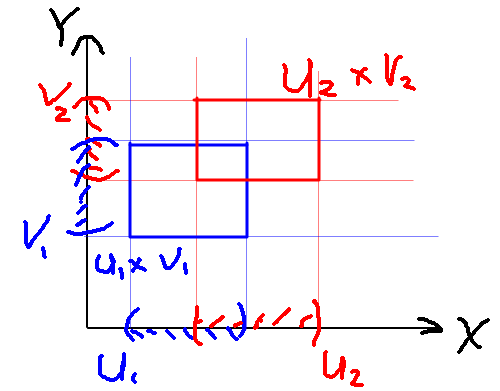
\includegraphics[scale=0.5]{product_topology_example} \\
			По рисунку видно, что верно только первое равенство
		\end{itemize}
		Как мы хотим задать топологию:
		$$
		\begin{rcases}
			U \sub X \text{ откр.} \\
			V \sub Y \text{ откр.}
		\end{rcases} \implies U \times V \text{ открыто в } (X \times Y) $$
		$ \mathcal{B} \define \set{U \times V | U \in \Omega_{X}, \Omega \in \Omega_Y} $ -- \textbf{не} топология (т. к. есть проблемы с объединением) \\
		Однако, $ \mathcal{B} $ -- база топологии
	\end{undefthm}
\end{eg}

\section{Прообраз топологии. Индуцированная топология}

\begin{definition}
	$ X $ -- множество, $ \qquad (Y, \Omega_Y) $ -- топ. пр-во, $ \qquad f : X \to Y $ \\
	Хотим ввести самую слабую топологию на $ X $, такую, чтобы $ f $ была непрерывной \\
	Такая топология называется прооразом топологии $ Y $
\end{definition}

\begin{proof}[корректности]
	Нужно доказать, что прообраз топологии существует и единственен \\
	$ f^{-1}(u) $ хотим считать открытыми, если $ U \in \Omega_Y $ \\
	$ \set{f^{-1}(U)} = \Omega_X $ -- топология на $ X $ (меньше взять не можем, больше -- не должны)
\end{proof}

\begin{definition}
	$ (X, \Omega) $ -- топ. пр-во, $ \qquad Y \sub X $ \\
	Определим $ \Omega_Y $:
	$$ \Omega_Y \define \set{U \cap Y | U \sub \Omega} $$
	$ \Omega_Y $ называется индуцированной топологией
\end{definition}

\begin{proof}[корректности]
	\hfill
	\begin{itemize}
		\item Проверим, что объединение открытых открыто:
		$$ \bigcup_{U_i \in \Omega} (U_i \cap Y) = \bigg( \bigcup_{U_i \in \Omega} U_i \bigg) \cap Y \sub \Omega_Y $$
		\item Проверим, что пересечение конечного набора открытых открыто:
		$$ \bigcap_{U_i \in \Omega} (U_i \cap Y) = \bigg( \bigcap_{U_i \in \Omega} U_i \bigg) \cap Y \sub \Omega_Y $$
		\item $ \O, Y \in \Omega_Y $
	\end{itemize}

\end{proof}

\section{Инициальная топология. Топология проиведения как инициальная}

\begin{definition}
	$ \set{(Y_i, \Omega_{Y_i})}_{i \in I} $ -- топ. пр-ва, $ \qquad X $ -- множество \\
	$ \forall i \quad $ задано отобр. $ f_ : X \to Y_i $ \\
	Хотим задать $ \Omega_X $ -- самую слабую, такую, чтобы все $ f_i $ были непрерывными
\end{definition}

\begin{proof}[коректности]
	Докажем, что инициальная топология существует и единственна: \\
	$ f^{-1}(U) $ будем считать открытым в $ X $ \\
	Положим $ \mathcal{B} \define \set{f_{ij}^{-1} U_{i1} \cap ... \cap f^{-1}_{ik} U_{ik}} $ -- база некоторой топологии на $ X $
\end{proof}

\begin{theorem}
	На $ X \times Y $ совпадают две топологии:
	\begin{itemize}
		\item как $ B = \set{U \times V} $ -- база
		\item инициальная
	\end{itemize}
\end{theorem}

\begin{proof}
	И та, и другая топологии определяются некоторой базой. Достаточно доказать, что базы совпадают \\
	Найдём базу инициалной топологии:
	$$ \mathcal{B} = \set{p_x^{-1}(U_1) \cap p_x^{-1}(U_2) \cap ... \cap p_x^{-1}(U_k) \quad \cap \quad p_y^{-1}(V_1) \cap p_y^{-1}(V_2) \cap ... \cap p_y^{-1}(V_l)} $$
	$$ p_x^{-1}(U) = \set{(x, y) | \underbrace{p_x(x, y)}_{= x} \in U} = U \times Y $$
	Аналогично, $ p_y^{-1}(V) = Y \times V $ \\
	Теперь,
	$$ \mathcal{B} = \underbrace{(U_1 \times Y) \cap (U_2 \times Y) \cap ... \cap (U_k \times Y)}_{(U_1 \cap ... \cap U_k) \times Y} \quad \cap \quad \underbrace{(X \times V_1) \cap (X \times V_2) \cap ... \cap (X \times V_l)}_{X \times (V_1 \cap ... \cap V_l)} $$
	$$ \mathcal{B} = (U_1 \cap U_2 \cap ... \cap U_k) \times (V_1 \cap V_2 \cap ... \cap V_l) $$
	Получили (открытые в $ X $) $ \times $ (открытые в $ Y $)
\end{proof}

\section{Финальная топология. Примеры}

\begin{definition}
	$ \set{(X_i, \Omega_i)}_{i \in I} $ -- топ. пр-ва, $ \qquad Y $ -- множество \\
	$ \forall i \quad $ задано $ f_i : X_i \to Y $ \\
	Хотим задать $ \Omega_Y $ -- самую сильную такую, что все $ f_i $ непрерывны
\end{definition}

\begin{statement}
	Несложно заметить, что подойдёт
	$$ \Omega_Y \define \set{U : \forall i \quad f_i^{-1}(U) \text{ откр. в } X} $$
\end{statement}

\section{Связность пространства и подмножества. Связность замыкания}

\begin{definition}
	$ X $ -- топ. пр-во \\
	$ X $ называется несвязным, если
	$$ \exist \underset{U_1, U_2 \ne \O}{U_1, U_2 \in \Omega_X} :
	\begin{cases}
		U_1 \cap U_2 = \O \\
		U_1 \cup U_2 = X
	\end{cases} $$
	Иначе -- связным
\end{definition}

\begin{remark}
	Несвязность $ \implies U_1, U_2 $ -- открытые и замкнутые одновременно \\
	Свзяность означает, что таких (нетривиальных открыто-замкнутых) нет
\end{remark}

\begin{definition}
	$ (X, \Omega) $ -- топ. пр-во, $ \quad A \sub X $ \\
	$ A $ называется связным, если оно связно в индуцированной топологии, т. е.
	$$ \forall U_1, U_2 \in \Omega_X \quad
	\begin{rcases}
		U_1 \cup U_2 \supset A \\
		U_1 \cap U_2 \cap A = \O
	\end{rcases} \implies \left[
	\begin{aligned}
		U_1 \cap A = \O \\
		U_2 \cap A = \O
	\end{aligned} \right. $$
\end{definition}

\begin{theorem}
	$ A $ связно, $ \quad A \sub B \sub \Cl A $ \\
	$ \implies B $ связно
\end{theorem}

\begin{proof}
	Пусть $ B $ не связно
	$$ \implies \exist U_1, U_2 \in \Omega_X :
	\begin{cases}
		U_1 \cup U_2 \supset B \\
		U_1 \cap U_2 \cap B = \O \\
		U_1 \cap B \ne \O \\
		U_2 \cap B \ne \O
	\end{cases} $$
	$$ A \sub B \implies
	\begin{cases}
		U_1 \cup U_2 \supset A \\
		U_1 \cap U_2 \cap A = \O
	\end{cases} \underimp{A \text{ связно}} \text{ НУО } A \cap U_1 = \O \implies U_2 \supset A $$
	Положим $ F \define \Cl A \setminus U_1 $ -- замкнутое, $ F \supset A \implies \Cl $ -- не минимальное -- \contra
\end{proof}

\begin{implication}
	$ A $ связно $ \implies \Cl A $ связно
\end{implication}

\section{Связность отрезка}

\begin{theorem}
	$ (0, 1) $ связен
\end{theorem}

\begin{proof}
	Пусть $ (0, 1) $ не связен
	$$ \implies \exist U_1, U_2 \text{ -- откр. } :
	\begin{cases}
		U_1 \cup U_2 \supset (0, 1) \\
		U_1 \cap U_2 \cap (0, 1) = \O
	\end{cases} $$
	Возьмём $ a \in U_1 \cap (0, 1), \qquad b \in U_2 \cap (0, 1) $ \\
	Будем считать, что $ a < b $ \\
	Т. к. $ (0, 1) $ не связен, между $ a $ и $ b $ есть проблемная точка. Найдём её:
	$$ x_* \define \sup\set{x \in U_1 | x < b} $$
	Почему эта точка проблемная?
	$$ \left[
	\begin{aligned}
		x_* \in U_1 \implies \exist \veps > 0 : (x_* - \veps, x_* + \veps) \sub U_1 \implies b > x_* + \veps \implies x_* \text{ не \textbf{верхняя} граница -- } \contra \\
		x_* \in U_2 \implies \exist \veps > 0 : (x_* - \veps, x_* + \veps) \sub U_2 \implies x_* \text{ не \textbf{точная} верхняя граница -- } \contra
	\end{aligned} \right. $$
	Значит, $ (0, 1) $ связен
\end{proof}

\begin{implication}
	$ [0, 1] $ связен (как замыкание $ (0, 1) $)
\end{implication}

\section{Связность объединения. Образ связного множества}

\begin{theorem}
	$ A, B $ связны, $ \quad A \cap B \ne \O $ \\
	$ \implies A \cup B $ связно
\end{theorem}

\begin{proof}
	Пусть $ U_1, U_2 \in \Omega :
	\begin{cases}
		U_1 \cup U_2 \sub (A \cup B) \\
		U_1 \cap U_2 \cap (A \cup B) = \O \\
		U_1 \cap (A \cup B) \ne \O \\
		U_2 \cap (A \cup B) \ne \O
	\end{cases} $ \\
	Возьмём $ x_0 \in A \cap B $ \\
	НУО считаем, что $
	\begin{cases}
		x_0 \in U_1 \\
		x_0 \notin U_2
	\end{cases} $
	$$
	\begin{rcases}
		U_1 \cup U_2 \supset A \\
		U_1 \cap U_2 \cap A = \O
	\end{rcases} \underimp{A \text{ связно}} \left[
	\begin{aligned}
		\cancel{U_1 \cap A = \O} \\
		U_2 \cap A = \O
	\end{aligned} \right. \underimp{x_0 \in A} U_2 \cap A = \O $$
	$$
	\begin{rcases}
		U_1 \cup U_2 \supset B \\
		U_1 \cap U_2 \cap B = \O
	\end{rcases} \underimp{B \text{ связно}} \left[
	\begin{aligned}
		\cancel{U_1 \cap B = \O} \\
		U_2 \cap B = \O
	\end{aligned} \right. \underimp{x_0 \in B} U_2 \cap B = \O $$
	$$
	\begin{rcases}
		U_2 \cap (A \cup B) \ne \O \\
		U_2 \cap A = \O \\
		U_2 \cap B = \O
	\end{rcases} \quad \contra $$
\end{proof}

\begin{theorem}
	$ f : X \to Y $ -- непр., $ \quad A $ -- связно \\
	$ \implies f(A) $ -- связно
\end{theorem}

\begin{proof}
	Пусть $ f(A) $ не связно \\
	Это означает, что $
	\begin{cases}
		f(A) \sub U_1 \cup U_2 \\
		U_1 \cap U_2 \cap f(A) = \O \\
		U_1 \cap f(A) \ni y_1 \\
		U_2 \cap f(A) \ni y_2
	\end{cases} $
	$$ V_1 \define f^{-1}(U_1), \qquad V_2 \define f^{-1}(U_2) $$
	$$ V_1 \cup V_2 = f^{-1}(U_1) \cup f^{-1}(U_2) = f^{-1}(U_1 \cup U_2) \supset f^{-1}(f(A)) \supset A $$
	$ V_1 \cap V_2 \cap A = \O $ (т. к. допустим, $ x_* \in V_1 \cap V_2 \cap A \implies f(x_*) \in U_1 \cap U_2 \cap f(A) = \O $)
\end{proof}

\begin{implication}
	$ X \simeq Y $ \\
	$ X $ связно $ \implies Y $ связно
\end{implication}

\section{Связность декартова произведения}

\begin{theorem}
	$ X \times Y $ связно $ \iff X, Y $ связно
\end{theorem}

\begin{proof}
	\hfill
	\begin{itemize}
		\item $ \implies $
		$$ \underset{p_x(x, y) = x}{p_x : X \times Y \to X}, \qquad \underset{p_y(x, y) = y}{p_y : X \times Y \to Y} $$
		Оба непрерывны
		\item Допустим, что $ X \times Y $ несвязно \\
		Тогда $ X \times Y = U_1 \cup U_2, \qquad U_1 \cap U_2 = \O $ \\
		Возьмём $ (x_1, y_1) \in U_1, \qquad (x_2, y_2) \in U_2 $ \\
		НУО считаем $ (x_1, y_2) \in U_1 $
	\end{itemize}

\end{proof}

\section{Теорема Вейерштрасса о промежуточном значении. Примеры применения}

\begin{statement}
	\begin{equ}{171}
		E \sub \R \text{ связно } \iff \forall x, y \in E \quad x < r < y \implies r \in E
	\end{equ}
\end{statement}

\begin{theorem}
	$ X $ -- топологическое пространство, связное \\
	$ f : X \to \R $ -- непрерывная функция, $ \qquad f(x_0) = a, \quad f(x_1) = b, \qquad a \le c \le b $
	$$ \implies \exist x_2 \in X : f(x_2) = c $$
\end{theorem}

\begin{proof}
	$ X $ -- связное $ \implies f(X) $ -- связное \\
	Для удобства, НУО предположим, что $ a < b $
	$$ a \le c \le b \underimp{\eref{171}} \exist x_2 : f(x_2) = c $$
\end{proof}

\section{Компоненты связности}

\begin{definition}[компонента связности точки]
	$$ K_a \define \bigcup_{
		\begin{subarray}{c}
			a \in A \\
			A \text{ связно}
		\end{subarray}} A \text{ -- связно} $$
\end{definition}

\begin{statement}
	$ K_a = K_b $ или $ K_a \cap K_b = \O $
\end{statement}

\begin{proof}
	Пусть $
	\begin{Bmatrix}
		K_a \ne K_b \\
		K_a \cap K_b \ne \O
	\end{Bmatrix} \implies K_a \cup K_b $ связно \\
	Получили множество, содержащее $ a $ и $ b $, большее, чем каждая из компонент -- \contra
\end{proof}

\begin{statement}
	$ K_a $ замкнута
\end{statement}

\begin{proof}
	Замыкание связного связно \\
	Если компонента связности не замкнута, то её замыкание тоже будет компонентой связноти, большей данной
\end{proof}

\begin{note}
	$ K_a $ не обязательно открыта
\end{note}

\begin{theorem}
	$ (X, \Omega) $ -- топологическое пространство. Равносильны следующие условия:
	\begin{enumerate}
		\item \label{en:181} Компоненты связности $ X $ открыты
		\item \label{en:182} $ X = \bigcup_{i \in I} X_i $, где $ X_i $ -- комп. связности \\
		Топология $ X $ совпадает с топологией объединения
		\item \label{en:183} У любой точки существует связная окрестность
	\end{enumerate}
\end{theorem}

\begin{proof}
	\textit{Здесь не будет строгого доказательства, потому что там много слов ни о чём}
	\begin{itemize}
		\item $ \ref{en:181} \iff \ref{en:183} $ \\
		Очевидно (эта окрестность и будет $ K_a $)
		\item $ \ref{en:182} $ \\
		Зададим топологию объединения как финальную:
		$$ \Omega_\cup \define \set{U : \operatorname{id}^{-1}(U) \text{ откр. в } X_i} $$
		Очевидно, что
		$$ \forall i \quad X_i \sub X \implies \exist \operatorname{id}^{-1}(X_i) = X_i $$
		Значит, $ X_i $ открыто
	\end{itemize}
\end{proof}

\section{Линейная связность}

\begin{definition}
	Путём в $ X $ называется непрерывное отображение $ f : [0, 1] \to X $
\end{definition}

\begin{definition}
	$ X $ называется линейно связным, если любые две точки соединены путём
\end{definition}

\begin{definition}
	$ A \sub X $ линейно связно, если любые две точки можно соединить путём в $ A $ (не выходящим за пределы $ A $)
\end{definition}

\begin{theorem}
	Линейно связное множество является связным
\end{theorem}

\begin{proof}
	Пусть не связно
	$$ \iff X = U_1 \cup U_2 :
	\begin{cases}
		U_1 \cap U_2 = \O \\
		x_1 \in U_1 \\
		x_2 \in U_2
	\end{cases} $$
	$$ \implies \exist f : [0, 1] \to X :
	\begin{cases}
		f(0) = x_1 \\
		f(1) = x_2
	\end{cases} $$
	$ f^{-1}(U_1), f^{-1}(U_2) $ разбивают отрезок $ [0, 1] \implies [0, 1] $ не связен -- \contra
\end{proof}

\begin{definition}
	Компонента линейной связности -- максимальное линейно связное подмножество
\end{definition}

\begin{statement}
	Компоненты лин. св. совпадают или не пересекаются
\end{statement}

\begin{note}
	Компоненты лин. св. не обязательно замкнуты
\end{note}

\section{Компактность. Примеры. Компактность замкнутого множества}

\begin{definition}
	$ X $ -- топ. пр-во \\
	$ \set{U_i}_{i \in I} $ называется открытым покрытием $ X $, если:
	\begin{enumerate}
		\item $ \bigcup_{i \in I} U_i = X $
		\item $ \forall i \quad U_i \in \Omega $
	\end{enumerate}
\end{definition}

Дальше слово покрытие будет обоначать ``открытое покрытие''

\begin{definition}
	$ \set{U_i}_{i \in I} $ -- покрытие $ X $
	Если $ \set{U_{i_j}}_{i_j \in J \sub I} $ -- тоже покрытие $ X $, то оно называется подпокрытием $ \set{U_i}_{i \in I} $
\end{definition}

\begin{definition}
	$ X $ называется компактным, если из любого покрытия можно выбрать конечное подпокрытие
\end{definition}

\begin{definition}
	$ A \sub X $ компактно, если оно компактно в индуцированной топологии, т. е.
	$$ \forall \underset{U_i \text{ откр. в } X}{\set{U_i}_{i \in I}} : \bigcup_{i \in I} U_i \supset A \quad \exist U_{i_1}, U_{i_2}, ..., U_{i_n} : \bigcup_{k = 1}^n U_{i_k} \supset A $$
\end{definition}

\begin{exmpls}
	\item Антидискретное \textbf{компактно} \\
	Любое его подмножество \textbf{компактно}
	\item Любое конечное топ. пр-во \textbf{компактно}
	\item Бесконечное дискретное \textbf{не компактно} \\
	(покрытие одноточечными мн-вами)
	\item $ \R_{\text{станд.}} $ \textbf{не компактно} \\
	($ U_n = (-n, n) $ -- покрытие, выкинуть ни один нельзя)
	\item Топология Зарисского \textbf{компактна}
	\item Стрелка:
	\begin{itemize}
		\item На $ [0, +\infty] $ -- \textbf{компактна}
		\item На $ (0, +\infty) $ -- \textbf{не компактна}
	\end{itemize}
\end{exmpls}

\begin{theorem}
	$ X $ компактно, $ \quad A $ замкнуто в $ X $
	$$ \implies A \text{ компактно} $$
\end{theorem}

\begin{proof}
	Рассмотрим $ \forall \set{U_i}_{i \in I} $ -- покрытие \\ $ A $
	Положим $ V \define X \setminus A $ -- откр. \\
	$ \set{U_i, V}_{i \in I} $ -- покр. $ X $ \\
	$ \implies \exist $ конечное подпокрытие. Выпишем его:
	$$ V, U_{i_1}, U_{i_2}, ..., U_{i_n} $$
	Тогда все $ U $ образуют конечное подпокрытие $ A $ (т. к. $ V \cap A = \O $)
\end{proof}

\section{Компактность образа компактного множества}

\begin{theorem}
	$ f : X \to Y $ -- непр., $ \quad A \sub X $ -- комп. \\
	$ \implies f(A) $ -- копм.
\end{theorem}

\begin{proof}
	Пусть $ \set{V_i \sub Y}_{i \in I} $ -- покрытие $ f(A) $ \\
	$ \implies \forall i \quad f^{-1}(V_i) $ -- откр. в $ X $ \\
	$ \implies \set{f^{-1}(V_i)}_{i \in I} $ -- покрытие $ A $ \\
	$ A $ компактно, поэтому можно выбрать конечное подпокрытие:
	$$ f^{-1}(V_{i_1}), ..., f^{-1}(V_{i_n}) \text{ -- кон. подпокр. } A $$
	$ V_{i_1}, ..., V_{i_m} $ -- кон. попокр. $ F(A) $
\end{proof}

\begin{implication}
	Компактность является топологическим свойством
\end{implication}

\section{Компактные подмножества хаусдорфова пространства}

\begin{definition}
	$ X $ называется хаусдорфовым, если любые две точки можно разделить непересекающимися окрестностями, т. е.
	$$ \forall \underset{x \ne y}{x, y \in X} \quad \exist U_x, U_y : U_x \cap U_y = \O $$
\end{definition}

\begin{theorem}
	$ X $ -- хаусдорфово, $ \quad A $ компактно \\
	$ \implies A $ замкнуто
\end{theorem}

\begin{proof}
	Нужно доказать, что $ X \setminus A $ открыто \\
	Зафиксируем $ x_0 \in X \setminus A $
	$$ X \text{ хаусд. } \implies \forall a \in A \quad \exist
	\begin{Bmatrix}
		U_{ax_0} \text{ -- окр. } a \\
		V_{ax_0} \text{ -- окр. } x_0
	\end{Bmatrix} : U \cap V = \O $$
	$ \set{U_{ax_0}}_{a \in A} $ -- покрытие $ A \implies \exist U_{ax_01}, ..., U_{ax_0n} $ -- конечное подпокрытие $ A $ \\
	Для каждой $ U_{ax_0i} $ возьмём парную ей $ V_{ax_0i} $:
	$$ V \define \bigcap_{k = 1}^n V_{ax_0k} $$
	$ V $ открыто, $ \quad V \cap A = \O $ (т. к. $ V_i \cap U_i = \O $), $ \quad x_0 \in V $
\end{proof}

\begin{implication}
	$ X $ -- компактно и хаусдорфово, $ \quad A \sub X $ \\
	$ A $ компактно $ \iff A $ замкнуто
\end{implication}

\section{Лемма Лебега. Компактность отрезка}

\begin{lemma}[Лебега]
	$ \set{U_i} $ -- покрытие $ [0, 1] $
	$$ \exist \underset{\text{число Лебега покрытия}}{\veps > 0} : \forall x_0 \in [0, 1] \quad \exist U_i : \underbrace{(x_0 - \veps, x_0 + \veps)}_{= B(x_0, \veps)} \cap I \sub U_i $$
\end{lemma}

\begin{remark}
	$ \veps $ не зависит от $ x_0 $
\end{remark}

\begin{proof}
	Положим $ \veps_i \define \dfrac1{2^i} $ ($ \veps_i \to 0 $) \\
	Пусть лемма невверна, т. е.
	$$ \exist x_i : \forall j \quad B(x_i, \veps_i) \not\sub U_j $$
	Применим принцип выбора Больцано-Вейерштрасса:
	$$ \exist x_{n_k} \to x_0 $$
	$$ x_0 \in U_j \implies \exist \underset{\text{из } veps_i \text{ в первой строчке}}{\veps_i} : B(x_0, \veps_i) \sub U_j $$
	Рассмотрим $ x_{n_k} : \rho(x_{n_k}, x_0) < \dfrac1{2i + 1} $ \\
	Пусть $ b_k \ge i + 1 $ (можно так сделать, т. к. последовательность сходится к $ x_0 $)
	$$ B(x_{n_k}, \veps_{n_k}) B(x_{n_k}, \veps_{i + 1}) \sub B(x_0, \veps_i) \sub U_j $$
	А мы предположили, что $ B(x_i, \veps_i) \not\sub U_j $ -- \contra
\end{proof}

\begin{theorem}
	$ [0, 1] $ компактен
\end{theorem}

\begin{proof}
	Пусть $ \set{U_i} $ -- открытое покрытие, $ \quad \veps $ -- его число Лебега \\
	Применим лемму Лебега:
	$$ [0, 1] \cap B(0, \veps) \sub U_0 $$
	$$ B(\veps, \veps) \sub U_1 $$
	$$ B(2\veps, \veps) \sub U_2 $$
	$$ \widedots[7em] $$
	$$ [0, 1] \cap B(k\veps, \veps) \sub U_k, \qquad (k + 1)\veps \ge 1 $$
	То есть, все эти шары покрывают отрезок \\
	Значит, $ U_1, ..., U_k $ -- конечное подпокрытие
\end{proof}

\section{Компактность произведения пространств}

\begin{theorem}
	$ X, Y $ комп. $ \iff X \times Y $ комп.
\end{theorem}

\begin{proof}
	\hfill
	\begin{itemize}
		\item $ \impliedby $ \\
		$ \underset{p_x(x, y) = x}{p_x} : X \times Y \to X $ -- непр. \\
		$ X \times Y $ -- комп. $ \implies p_x(X \times Y) = X $ -- комп. \\
		Аналогично для $ Y $ и $ p_y $
		\item $ \implies $ \\
		Возьмём $ \set{U_i \times V_i} $ -- покрытие $ X \times Y $ \\
		Рассмотрим $ x_0 \in X $ и слой над ней: $ \set{x_0} \times Y \simeq Y $
		$ \set{x_0} \times Y $ -- комп. $ \implies \exist \set{U_{ix_0}  \times V_{ix_0}}_{i = 1}^{n_{x_0}} $ -- покрытие
		$$ U_{x_0} \define \bigcap_{i = 1}^n U_{ix_0} \text{ -- откр.} $$
		Теперь будем менять $ x_0 $: \\
		$ \set{U_{x_0}}_{x_0 \in X} $ -- открытое покрытие $ X $ \\
		$ X $ -- комп. $ \implies U_{x_1}, ..., U_{x_m} $ -- конечное подпокрытие \\
		$ \set{U_{ix_1} \times V_{ix_1}}_{i = 1}^{n_{x_1}}, \widedots[4em], \set{U_{ix_m} \times V_{ix_m}}_{i = 1}^{n_{x_m}} $ -- конечное подпокрытие
	\end{itemize}

\end{proof}

\begin{remark}
	Верна теорема Тихонова: \\
	$ X_i $ -- комп. $ \iff \prod X_i $ -- комп.
\end{remark}

\section({Критерий компактности в R\textasciicircum{}n}){Критерий компактности в $ \bm{\R^n} $}

\begin{definition}
	$ A \sub R^n $ ограничено, если $ \exist M > 0 : A \sub B(0, M) $ \\
	Или: $ S \sub [-M, M]^n $
\end{definition}

\begin{theorem}
	$ A \sub \R^n $ \\
	$ A $ компактно $ \iff A $ замкнуто и ограничено
\end{theorem}

\begin{proof}
	\hfill
	\begin{itemize}
		\item $ \implies $
		\begin{itemize}
			\item Замкнутость:
			$$
			\begin{rcases}
				\R^n \text{ хаусдорфово} \\
				A \text{ компактно}
			\end{rcases} \implies A \text{ замкнуто} $$
			\item Ограниченность: \\
			Иначе $ \set{B(0, M)}_{M = 1}^\infty $ -- покрытие без конечного подпокрытия
		\end{itemize}
		\item $ \impliedby $ \\
		$ [-M, M] $ комп. ($ \simeq [0, 1] $) $ \implies [-M, M]^n $ -- комп. (как прямое произведение)
		$$
		\begin{rcases}
			A \text{ замкнуто} \\
			A \sub [-M, M]^n
		\end{rcases} \implies A \text{ комп.} $$
	\end{itemize}
\end{proof}

\section{Теорема Вейерштрасса о достижении максимума. Примеры \texorpdfstring{\\}{} применения}

\begin{theorem}
	$ f : X \to \R $ -- непр., $ \quad X $ -- комп.
	$$ \implies \exist x_0 : \forall x_1 \quad f(x_1) \le f(x_0) $$
\end{theorem}

\begin{proof}
	$ X $ -- комп. $ \implies f(X) \sub \R $ -- комп. \\
	Знаем, что компактные подмножества прямой замкнуты и ограничены, а значит, $ \exist \max(f(x)) $
\end{proof}

\begin{eg}[метод Штурма]
	$$ \frac{x_1 + x_2 + ... + x_n}n \ge \sqrt[n]{x_1x_2...x_n} $$
\end{eg}

\begin{proof}
	Докажем его следующим методом (в предположении, что $ x_i \ge 0 $):
	$$ S \define x_1 + x_2 + ... + x_n $$
	$$ M \define \set{(x_1 \cdot ... \cdot x_n) \in \R^n |
		\begin{cases}
			x_i \ge 0 \\
			\sum_{i = 1}^n x_i = S
		\end{cases}} $$
	$$ f(x_1, ..., x_n) \define x_1x_2...x_n, \qquad f : M \to \R $$
	Утверждается, что если $ x_1 = x_2 = ... = x_n = \frac{S}n $, то $ f(\frac{S}n, \frac{S}n, ..., \frac{S}n) \stackrel?\ge f(x_1, x_2, ..., x_n) $
	Докажем, что это максимум. Для этого докажем, что остальные точки не являются максимумом: \\
	Пусть $ x_i < x_j $ \\
	Выберем $ \veps < \dfrac{x_i - x_j}2 $ \\
	Утверждается, что $ x_ix_j < (x_i + \veps)(x_j - \veps) $ \\
	Докажем это:
	$$ (x_i + \veps)(x_j - \veps) = x_ix_j + \veps \underbrace{(x_j - x_i - \veps)}_{> 0} $$
	Получили, что любой набор $ \set{x_i} $, кроме одинаковых, улучшаем (при фиксированной сумме) \\
	Если максимум существует, то это одинаковые $ x_i $ \\
	Докажем его существование:
	$ M $ -- комакт (т. к. это -- замкнутое ограниченное подмножество $ \R^n $) $ \underimp{\text{т. В.}} f $ имеет максимум
\end{proof}

\begin{eg}[задача Фаньяна]
	Есть остроугольный треугольник $ ABC $. Хотим вписать в него треугольник $ XYZ $ так, чтобы $ P(XYZ) \to \min $ \\
	Утверждается, что $ X, Y, Z $ -- основания высот \\
	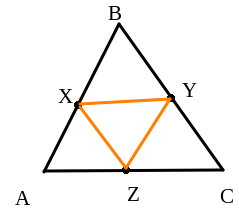
\includegraphics{faryan_problem_1}
\end{eg}

\begin{proof}
	$$ \set{(X, Y, Z)} = AB \times BC \times CA \text{ -- комп.} $$
	Значит, существует такая конфигурация $ X, Y, Z $, что $ P(XYZ) = \max $ \\
	Утверждается, что единственная неулучшаемая концигурация:
	$$
	\begin{cases}
		\angle BXY = \angle BYX \\
		\angle AXZ = \angle AZX \\
		\angle YCZ = \angle ZCY
	\end{cases} $$
	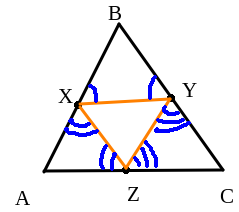
\includegraphics{faryan_problem_2} \\
	Докажем это: \\
	Пусть $ \angle AZX < \angle CZY $, при этом, $ \angle AZ_0X = \angle CZ_0Y $ \\
	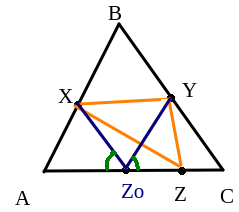
\includegraphics{faryan_problem_3} \\
	Вспоминая прошлый семестр, это означает, что $ XZ_0 + YZ_0 < XZ + YZ $
\end{proof}

\begin{eg}[задача Дидоны]
	Требуется найти фигуру с максимальной площадью при заданном периметре \\
	Утверждается, что это круг
\end{eg}

\begin{proof}
	Пусть $ M $ -- множество выпуклых фигур с периметром $ P $ \\
	$ f $ -- функция площади \\
	Единственная неулучшаемая фигура -- круг \\
	Значит, достаточно доказать, что $ M $ компактно \\
	Хотим превратить $ M $ в топологическое пространство, так, чтобы функция площади была непрерывна \\
	Введём для этого метрику. Нам подойдёт метрика Хаусдорфа
	\begin{undefthm}{В каких случаях $ \bm{M} $ может не быть компактом?}
		\item Рассмотрим в качестве $ M $ множество фигур на плоскости. Это (почти всегда) \textbf{не} компакт (т. к. фигуры можно сдвигать сколь угодно далеко)
	\end{undefthm}
	Возьмём в качестве $ M $ множество фигур в каком-нибудь ограниченном множестве (например, в квадрате со стороной $ P $) \\
	Метрика -- метрика Хаусдорфа \\
	Утверждается, что таким образом построенное множество компактно (без доказательства)
\end{proof}

\section{Аксиомы отделимости. Критерий T1}

\begin{statements}
	$ X $ -- топологическое пространство. $ X $ может удовлетворять следующим аксиомам:
	\begin{enumerate}
		\item[$ \bm{T_0} $] (Колмогорова). Для любых двух различных точек существует окрестность, содержащая ровно одну из них
		\item[$ \bm{T_1} $] (Тихонова). $ \forall \underset{x \ne y}{x, y \in X} \quad \exist U_x \not\ni y $
		\item[$ \bm{T_2} $] (Хаусдорфа). $ \forall \underset{x \ne y}{x, y \in X} \quad \exist \underset{\ni x}{U_x}, \underset{\ni y}{U_y} : U_x \cap U_y = \O $
		\item[$ \bm{T3} $]. $ \forall F $ -- замкн. $ \quad \forall x \notin F \quad \exist $ открытые $ \underset{\ni x}{U_x}, \underset{\supset F}{U_F} ~ : ~ U_x \cap U_F = \O $
		\item[$ \bm{T4} $]. $ \forall \underset{F_1 \cap F_2 = \O}{F_1, F_2 \text{ -- замкн.}} \quad \exist $ открытые $ \underset{\supset F_1}{U_1}, \underset{\supset F_2}{U_2} ~ : ~ U_1 \cap U_2 = \O $
	\end{enumerate}
\end{statements}

\begin{remark}
	$ \bm{T_2} \implies \bm{T_1} \implies \bm{T_0} $
\end{remark}

\begin{theorem}
	$ \bm{T_1} \iff $ любая точка -- замкнутое множество
\end{theorem}

\begin{proof}
	\hfill
	\begin{itemize}
		\item $ \implies $
		$$ \bm{T_1} \iff \forall x_0 \in X \quad \forall \underset{y \ne x_0}{y \in X} \quad \exist U_y :
		\begin{cases}
			y \in U_y \\
			x_0 \notin U_y
		\end{cases} $$
		$$ \bigcup_{y \in X \setminus \set{x_0}} U_y = X \setminus \set{x_0} \underset{\text{(как объединение открытых)}}{\text{ -- откр. }} \implies \set{x_0} \text{ -- замкн.} $$
		\item $ \impliedby $
		$$ \forall x \ne y \quad U_x \define X \setminus \set{y} \underset{\text{(т. к. } y \text{ замкн.)}}{\text{ -- откр.}} $$
		Получили окрестность, которая содержит $ x $, но не содержит $ y $
	\end{itemize}
\end{proof}

\begin{implication}
	При $ \bm{T_1} $ верно, что $ \bm{T_4} \implies \bm{T_3} \implies \bm{T_2} \implies \bm{T_1} $
\end{implication}

\section{Нормальность метрического пространства}

\begin{definition}
	Пространство, удовлетворяющее $ \bm{T_1} $ и $ \bm{T_3} $ (по следствию, $ \bm{T_0} $ -- $ \bm{T_3} $) называется регулярным
\end{definition}

\begin{definition}
	Пространство, удовлетворяющее $ \bm{T_1} $ и $ \bm{T_4} $ (по следствию, $ \bm{T_0} $ -- $ \bm{T_4} $) называется нормальным
\end{definition}

\begin{theorem}
	Метрическое пространство нормально
\end{theorem}

\begin{theorem}
	\hfill
	\begin{itemize}
		\item Хаусдорфовость ($ \bm{T_2} $): \\
		Возьмём $ x \ne y, \qquad \veps \define \dfrac{\rho(x, y)}2 $
		$$ B(x, \veps) \cap B(y, \veps) \stackrel{\vartriangle}= \O $$
		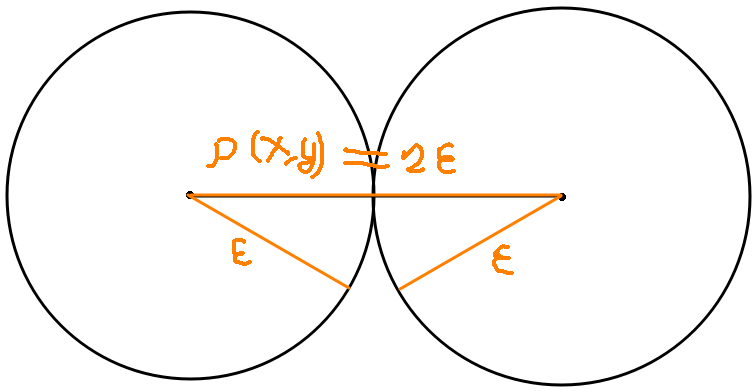
\includegraphics[scale=0.4]{norm_metr}
		\item Регулярность ($ \bm{T_3} $):
		Возьмём $ x_0 \in X, \quad F $ -- замкн.
		$$ \implies \exist \rho(x_0, F) \define \inf\limits_{y \in F} \rho(x, y) \stackrel?> 0 $$
		Пусть $ \inf\limits_{y \in F} \rho(x_0, y) = 0 $
		\begin{multline*}
			\implies \exist y_n : \rho(x_0, y_n) \underarr{n \to \infty} 0 \bydef[\iff] \forall \veps > 0 \quad \exist N : \forall n > N \quad y_n \in B(x_0, \veps) \implies \\
			\implies x_0 \in \Cl\set{y_n} \sub \Cl F \underset{(F \text{ замкнуто})}= F
		\end{multline*}
		Положим $ \veps \define \dfrac{\rho(x_0, F)}2 $ \\
		Возьмём $ U_{x_0} \define B(x_0, \veps) $ и $ U_F \define \bigcup_{y \in F} B(y, \veps) $ -- открыты (т. к. шары открыты)
		\item $ \bm{T_4} $ \\
		$ F_1, F_2 $ -- замкнутые. Хотим, чтобы $ \rho(F_1, F_2) $ могло равняться нулю \\
		Пусть это не так:
		$$
		\begin{cases}
			\forall x \in F_1 \quad \exist \veps_x \define \frac{\rho(x, F_2)} > 0 \\
			\forall y \in F_2 \quad \exist \veps_y \define \frac{\rho(y, F_1)} > 0
		\end{cases} $$
		$$ U_{F_1} \define \bigcup_{x \in F_1} B(x, \veps_x), \qquad U_{F_2} \define \bigcup_{y \in F_2} B(y, \veps_y) $$
		$$ x \in (U_{F_1} \cap U_{F_2} ) \implies x \in \bigg( B(x, \veps_x) \cap B(y, \veps_y) \bigg) $$
		Пусть, НУО, $ \veps_x \ge \veps_y $
		$$ \implies \rho(x, y) < 2 \veps_x = \rho(x, F_2) $$
		Вспомним, что $ x \in F_1, y \in F_2 $ \\
		Получили, что расстояние от $ x $ до некоторой точки фигуры $ F_2 $ больше, чем до самой $ F_2 $ - \contra
	\end{itemize}

\end{theorem}

\section{Нормальность хаусдорфова компакта}

\begin{theorem}
	$ X $ -- компактно и хаусдорфово $ \implies X $ нормально
\end{theorem}

\begin{proof}
	\hfill
	\begin{itemize}
		\item Регулярность ($ \bm{T_0} $ -- $ \bm{T_3} $) \\
		Возьмём $ x_0 \in X $ и $ F $ -- замкнутое в $ X $ ($ \implies F $ компактно, в силу хаусдорфовости $ X $) \\
		В силу хаусдорфовости $ F $,
		$$ \forall y \in F \quad \exist
		\begin{Bmatrix}
			U_{x_0, y} \text{ -- откр.} \\
			V_y \text{ -- откр.}
		\end{Bmatrix} : U_{x_0, y} \cap V_y = \O $$
		Возьмём $ \set{V_y}_{y \in F} $ -- конечное покрытие $ F $
		$$ \implies \exist V_{y_1}, ..., V_{y_n} \in F \text{ -- конечное подпокрытие } F $$
		$$ U_{x_0} \define \bigcap_{i = 1}^n U_{x_0, y_i} \text{ -- откр.}, \qquad U_F \define \bigcap_{i = 1}^n V_{y_i} $$
		\item Нормальность ($ \bm{T_4} $) \\
		Заданы $ F_1, F_2 $ -- замкнутые непересекающиеся множества \\
		Возьмём $ x \in F_1, \quad \underset{\text{окр. } x}{U_x}, \quad \underset{\text{окр. } F_2}{V_x} : U_x \cap V_x = \O $ (можно так сделать в силу $ \bm{T_3} $) \\
		Воспользуемся компактностью $ F_1 $ (как подмножества $ X $): \\
		Возьмём $ \set{U_x}_{x \in F_1} $ -- покрытие $ F_1 $ \\
		Значит, существует $ \set{U_{x_i}}_{i = 1}^k $ -- подпокрытие $ F_1 $
		$$ U_{F_1} \define \bigcup_{i = 1}^n U_{x_i}, \qquad U_{F_2} \define \bigcap_{i = 1}^n V_{x_i} $$
	\end{itemize}

\end{proof}

\section{Компактификация по П. С. Александрову}

\begin{definition}
	$ X $ называется локально компактным, если у любой точки есть окрестность с компактным замыканием, т. е.
	$$ \forall x_0 \in X \quad \exist U_{x_0} : \Cl U_{x_0} \text{ -- комп.} $$
\end{definition}


\begin{theorem}
	$ X $ локально компактно и хаусдорфово
	$$ \implies \exist \hat{X} \define X \cup \set{\infty} $$
	$ X $ -- подпространство $ \hat{X} $ \\
	$ \hat{X} $ компактно и хаусдорфово
\end{theorem}

\begin{proof}
	По условию, $ \hat{X} = X \cup \set{\infty} $ \\
	Открытые в $ \hat{X} $:
	\begin{itemize}
		\item $ \infty \in U $ \\
		$ U $ открыто в $ \hat{X} \iff U $ открыто в $ X $
		\item $ \infty \in U $ \\
		$ U $ открыто в $ \hat{X} \iff \underset{( = X \setminus U)}{\hat{X} \setminus U} $ компактно
	\end{itemize}
	\begin{itemize}
		\item[\textopenbullet] Докажем, что $ X $ -- подпространство $ \hat{X} $: \\
		Достаточно доказать, что если $ \infty \in U $, то $ (U \setminus \set{\infty}) $ открыто в $ X $
		$$ X \setminus \big( U \setminus \set{\infty} \big) \text{ комп. в } X \underimp{X \text{ -- хаусд.}} X \setminus \big( U \setminus \set{\infty} \big) \text{ замкнуто } \implies \big( U \setminus \set{\infty} \big) \text{ открыто} $$
		\item[\textopenbullet] Очевидно, что $ \hat{X} $ компактно
		\item[\textopenbullet] Докажем, что $ \hat{X} $ хаусдорфово:
		\begin{itemize}
			\item $ x_0, y_0 \in \big( \hat{X} \setminus \set{\infty} \big) \implies $ ОК (разделяем в $ X $)
			\item НУО $ x_0 \in \big( \hat{X} \setminus \set{\infty} \big), \quad y_0 = \infty $ \\
			В силу локальной компактности $ X $,
			$$ \exist U_{x_0} \sub X : \Cl U_{x_0} \text{ -- комп.} $$
			$$ U_{y_0} \define \big( X \setminus \Cl U_{x_0}) \text{ -- откр. в } \hat{X} \text{ и содержит } y_0 = \infty $$
		\end{itemize}

	\end{itemize}


\end{proof}
